% This LaTeX document needs to be compiled with XeLaTeX.
\documentclass[10pt]{article}
\usepackage[utf8]{inputenc}
\usepackage{amsmath}
\usepackage{amsfonts}
\usepackage{amssymb}
\usepackage[version=4]{mhchem}
\usepackage{stmaryrd}
\usepackage{graphicx}
\usepackage[export]{adjustbox}
\graphicspath{ {./images/} }
\usepackage{bbold}
\usepackage[fallback]{xeCJK}
\usepackage{polyglossia}
\usepackage{fontspec}
\IfFontExistsTF{Noto Serif CJK TC}
{\setCJKmainfont{Noto Serif CJK TC}}
{\IfFontExistsTF{STSong}
  {\setCJKmainfont{STSong}}
  {\IfFontExistsTF{Droid Sans Fallback}
    {\setCJKmainfont{Droid Sans Fallback}}
    {\setCJKmainfont{SimSun}}
}}

\setmainlanguage{english}
\IfFontExistsTF{CMU Serif}
{\setmainfont{CMU Serif}}
{\IfFontExistsTF{DejaVu Sans}
  {\setmainfont{DejaVu Sans}}
  {\setmainfont{Georgia}}
}

\begin{document}
\section*{MATHEMATICS}
\section*{SECTION-A}
\begin{enumerate}
  \setcounter{enumi}{60}
  \item \(\lim _{\mathrm{n} \rightarrow \infty}\left(\frac{1}{1+\mathrm{n}}+\frac{1}{2+\mathrm{n}}+\frac{1}{3+\mathrm{n}}+\ldots+\frac{1}{2 \mathrm{n}}\right)\) is equal to :-\\
(1) 0\\
(2) \(\log _{\mathrm{e}} 2\)\\
(3) \(\log _{\mathrm{e}}\left(\frac{3}{2}\right)\)\\
(4) \(\log _{\mathrm{e}}\left(\frac{2}{3}\right)\)
\end{enumerate}

Official Ans. by NTA (2)\\
Allen Ans. (2)\\
Sol. \(\lim _{n \rightarrow \infty}\left(\frac{1}{1+n}+\ldots+\frac{1}{n+n}\right)=\lim _{n \rightarrow \infty} \sum_{r=1}^{n} \frac{1}{n+r}\)

\[
\begin{aligned}
& =\lim _{\mathrm{n} \rightarrow \infty} \sum_{\mathrm{r}=1}^{\mathrm{n}} \frac{1}{\mathrm{n}}\left(\frac{1}{1+\frac{\mathrm{r}}{\mathrm{n}}}\right) \\
& =\int_{0}^{1} \frac{1}{1+\mathrm{x}} \mathrm{dx}=\left[\ell \mathrm{n}(1+\mathrm{x}]_{0}^{1}=\ell \mathrm{n} 2\right.
\end{aligned}
\]

\begin{enumerate}
  \setcounter{enumi}{61}
  \item The negation of the expression \(q \vee((\sim q) \wedge p)\) is equivalent to\\
\((1)(\sim p) \wedge(\sim q)\)\\
(2) \(\mathrm{p} \wedge(\sim \mathrm{q})\)\\
(3) \((\sim p) \vee(\sim q)\)\\
(4) \((\sim p) \vee q\)
\end{enumerate}

Official Ans. by NTA (1)\\
Allen Ans. (1)\\
Sol. \(\quad \sim(q \vee((\sim q) \wedge p))\)\\
\(=\sim q \wedge \sim((\sim q) \wedge p)\)\\
\(=\sim q \wedge(q \vee \sim p)\)\\
\(=(\sim q \wedge q) \vee(\sim q \wedge \sim p)\)\\
\(=(\sim q \wedge \sim p)\)\\
63. In a binomial distribution \(B(n, p)\), the sum and product of the mean \& variance are 5 and 6 respectively, then find \(6(n+p-q)\) is equal to :-\\
(1) 51\\
(2) 52\\
(3) 53\\
(4) 50

Official Ans. by NTA (2)\\
Allen Ans. (2)

\section*{TEST PAPER WITH SOLUTION}
Sol. \(\quad n p+n p q=5, n p . n p q=6\)\\
\(n p(1+q)=5, n^{2} p^{2} q=6\)\\
\(\mathrm{n}^{2} \mathrm{p}^{2}(1+\mathrm{q})^{2}=25, \mathrm{n}^{2} \mathrm{p}^{2} \mathrm{q}=6\)\\
\(\frac{6}{\mathrm{q}}(1+\mathrm{q})^{2}=25\)\\
\(6 q^{2}+12 q+6=25 q\)\\
\(6 q^{2}-13 q+6=0\)\\
\(6 q^{2}-9 q-4 q+6=0\)\\
\((3 q-2)(2 q-3)=0\)\\
\(\mathrm{q}=\frac{2}{3}, \frac{3}{2}, \mathrm{q}=\frac{2}{3}\) is accepted\\
\(\mathrm{p}=\frac{1}{3} \Rightarrow \mathrm{n} \cdot \frac{1}{3}+\mathrm{n} \cdot \frac{1}{3} \cdot \frac{2}{3}=5\)\\
\(\frac{3 n+2 n}{9}=5\)\\
\(\mathrm{n}=9\)\\
So \(6(n+p-q)=6\left(9+\frac{1}{3}-\frac{2}{3}\right)=52\)\\
64. The sum to 10 terms of the series \(\frac{1}{1+1^{2}+1^{4}}+\frac{2}{1+2^{2}+2^{4}}+\frac{3}{1+3^{2}+3^{4}}+\ldots\). is:-\\
(1) \(\frac{59}{111}\)\\
(2) \(\frac{55}{111}\)\\
(3) \(\frac{56}{111}\)\\
(4) \(\frac{58}{111}\)

Official Ans. by NTA (2)\\
Allen Ans. (2)\\
Sol. \(\mathrm{T}_{\mathrm{r}}=\frac{\left(\mathrm{r}^{2}+\mathrm{r}+1\right)-\left(\mathrm{r}^{2}-\mathrm{r}+1\right)}{2\left(\mathrm{r}^{4}+\mathrm{r}^{2}+1\right)}\)

\[
\begin{aligned}
\Rightarrow \mathrm{T}_{\mathrm{r}} & =\frac{1}{2}\left[\frac{1}{\mathrm{r}^{2}-\mathrm{r}+1}-\frac{1}{\mathrm{r}^{2}+\mathrm{r}+1}\right] \\
T_{1} & =\frac{1}{2}\left[\frac{1}{1}-\frac{1}{3}\right] \\
T_{2} & =\frac{1}{2}\left[\frac{1}{3}-\frac{1}{7}\right]
\end{aligned}
\]

\[
\begin{gathered}
T_{3}=\frac{1}{2}\left[\frac{1}{7}-\frac{1}{13}\right] \\
\vdots \\
\mathrm{T}_{10}=\frac{1}{2}\left[\frac{1}{91}-\frac{1}{111}\right] \\
\Rightarrow \sum_{\mathrm{r}=1}^{10} \mathrm{~T}_{\mathrm{r}}=\frac{1}{2}\left[1-\frac{1}{111}\right]=\frac{55}{111}
\end{gathered}
\]

\begin{enumerate}
  \setcounter{enumi}{64}
  \item The value of \(\frac{1}{1!50!}+\frac{1}{3!48!}+\frac{1}{5!46!}+\ldots .+\frac{1}{49!2!}+\frac{1}{51!1!}\) is\\
(1) \(\frac{2^{50}}{50!}\)\\
(2) \(\frac{2^{50}}{51!}\)\\
(3) \(\frac{2^{51}}{51!}\)\\
(4) \(\frac{2^{51}}{50!}\)
\end{enumerate}

Official Ans. by NTA (2)\\
Allen Ans. (2)\\
Sol. \(\sum_{r=1}^{26} \frac{1}{(2 r-1)!(51-(2 r-1))!}=\sum_{r=1}^{26}{ }^{51} \mathrm{C}_{(2 r-1)} \frac{1}{51!} =\frac{1}{51!}\left\{{ }^{51} \mathrm{C}_{1}+{ }^{51} \mathrm{C}_{3}+\ldots .+{ }^{51} \mathrm{C}_{51}\right\}=\frac{1}{51!}\left(2^{50}\right)\)\\
66. If the orthocentre of the triangle, whose vertices are ( 1,2 ), ( 2,3 ) and ( 3,1 ) is ( \(\alpha, \beta\) ), then the quadratic equation whose roots are \(\alpha+4 \beta\) and \(4 \alpha+\beta\), is\\
(1) \(\mathrm{x}^{2}-19 \mathrm{x}+90=0\)\\
(2) \(x^{2}-18 x+80=0\)\\
(3) \(x^{2}-22 x+120=0\)\\
(4) \(x^{2}-20 x+99=0\)

Official Ans. by NTA (4)\\
Allen Ans. (4)\\
Sol.\\
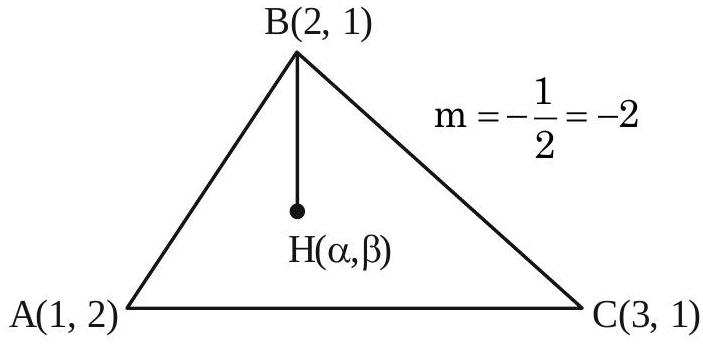
\includegraphics[max width=\textwidth, center]{2025_10_03_d195c8d2898bd93b94b0g-2(1)}

\[
\mathrm{m}=-\frac{1}{2}
\]

Here \(\mathrm{mBH} \times \mathrm{mAC}=-1\)\\
\(\left(\frac{\beta-3}{\alpha-2}\right)\left(\frac{1}{-2}\right)=-1\)\\
\(\beta-3=2 \alpha-4\)\\
\(\beta=2 \alpha-1\)\\
\(\mathrm{m}_{\mathrm{AH}} \times \mathrm{m}_{\mathrm{BC}}=-1\)\\
\(\Rightarrow \quad\left(\frac{\beta-2}{\alpha-1}\right)(-2)=-1\)\\
\(\Rightarrow \quad 2 \beta-4=\alpha-1\)\\
\(\Rightarrow \quad 2(2 \alpha-1)=\alpha+3\)\\
\(\Rightarrow \quad 3 \alpha=5\)\\
\(\alpha=\frac{5}{3}, \beta=\frac{7}{3} \Rightarrow \mathrm{H}\left(\frac{5}{3}, \frac{7}{3}\right)\)\\
\(\alpha+4 \beta=\frac{5}{3}+\frac{28}{3}=\frac{33}{3}=11\)\\
\(\beta+4 \alpha=\frac{7}{3}+\frac{20}{3}=\frac{27}{3}=9\)\\
\(x^{2}-20 x+99=0\)\\
67. For a triangle ABC , the value of \(\cos 2 \mathrm{~A}+\cos 2 \mathrm{~B}+\cos 2 \mathrm{C}\) is least. If its inradius is 3 and incentre is M , then which of the following is NOT correct?\\
(1) Perimeter of \(\triangle \mathrm{ABC}\) is \(18 \sqrt{3}\)\\
(2) \(\sin 2 \mathrm{~A}+\sin 2 \mathrm{~B}+\sin 2 \mathrm{C}=\sin \mathrm{A}+\sin \mathrm{B}+\sin \mathrm{C}\)\\
(3) \(\overrightarrow{\mathrm{MA}} \cdot \overrightarrow{\mathrm{MB}}=-18\)\\
(4) area of \(\triangle \mathrm{ABC}\) is \(\frac{27 \sqrt{3}}{2}\)

Official Ans. by NTA (4)\\
Allen Ans. (4)\\
Sol.\\
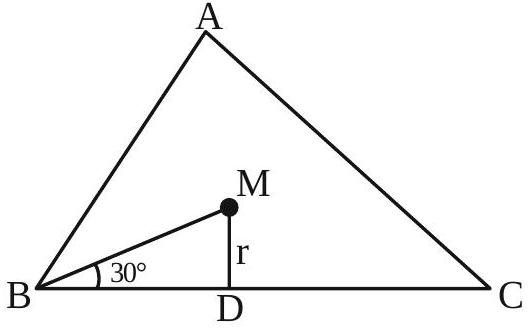
\includegraphics[max width=\textwidth, center]{2025_10_03_d195c8d2898bd93b94b0g-2}

If \(\cos 2 \mathrm{~A}+\cos 2 \mathrm{~B}+\cos 2 \mathrm{C}\) is minimum then \(\mathrm{A}= \mathrm{B}=\mathrm{C}=60^{\circ}\)

So \(\triangle \mathrm{ABC}\) is equilateral\\
Now in-radias \(\mathrm{r}=3\)\\
So in \(\triangle \mathrm{MBD}\) we have\\
\(\operatorname{Tan} 30^{\circ}=\frac{M D}{B D}=\frac{r}{a / 2}=\frac{6}{a}\)\\
\(1 / \sqrt{3}=\frac{1}{a}=a=6 \sqrt{3}\)\\
Perimeter of \(\triangle \mathrm{ABC}=18 \sqrt{3}\)\\
Area of \(\Delta \mathrm{ABC}=\frac{\sqrt{3}}{4} a^{2}=27 \sqrt{3}\)\\
68. The combined equation of the two lines \(\mathrm{ax}+\mathrm{by}+\mathrm{c}=0\) and \(\mathrm{a}^{\prime} \mathrm{x}+\mathrm{b}^{\prime} \mathrm{y}+\mathrm{c}^{\prime}=0\) can be written as \((a x+b y+c)\left(a^{\prime} x+b^{\prime} y+c^{\prime}\right)=0\)\\
The equation of the angle bisectors of the lines represented by the equation \(2 x^{2}+x y-3 y^{2}=0\) is\\
(1) \(3 x^{2}+5 x y+2 y^{2}=0\)\\
(2) \(x^{2}-y^{2}+10 x y=0\)\\
(3) \(3 x^{2}+x y-2 y^{2}=0\)\\
(4) \(x^{2}-y^{2}-10 x y=0\)

Official Ans. by NTA (4)\\
Allen Ans. (4)\\
Sol.\\
Equation of the pair of angle bisector for the homogenous equation \(a x^{2}+2 h x y+b y^{2}=0\) is given as\\
\(\frac{x^{2}-y^{2}}{a-b}=\frac{x y}{h}\)\\
Here \(\mathrm{a}=2, \mathrm{~h}=1 / 2 \& \mathrm{~b}=-3\)\\
Equation will become\\
\(\frac{x^{2}-y^{2}}{2-(-3)}=\frac{x y}{1 / 2}\)\\
\(x^{2}-y^{2}=10 x y\)\\
\(x^{2}-y^{2}-10 x y=0\)\\
69. The shortest distance between the lines \(\frac{x-5}{1}=\frac{y-2}{2}=\frac{z-4}{-3}\) and \(\frac{x+3}{1}=\frac{y+5}{4}=\frac{z-1}{-5}\) is\\
(1) \(7 \sqrt{3}\)\\
(2) \(5 \sqrt{3}\)\\
(3) \(6 \sqrt{3}\)\\
(4) \(4 \sqrt{3}\)

Official Ans. by NTA (3)\\
Allen Ans. (3)

Sol.\\
Shortest distance between two lines\\
\(\frac{x-x_{1}}{a_{1}}=\frac{y-y_{1}}{a_{2}}=\frac{z-z_{1}}{a_{3}}\) \&\\
\(\frac{x-x_{2}}{b_{1}}=\frac{y-y_{2}}{b_{2}}=\frac{z-z_{2}}{b_{3}}\) is given as\\
\(\frac{\left|\begin{array}{ccc}x_{1}-x_{2} & y_{1}-y_{2} & z_{1}-z_{2} \\ a_{1} & a_{2} & a_{3} \\ b_{1} & b_{2} & b_{3}\end{array}\right|}{\sqrt{\left(a_{1} b_{3}-a_{3} b_{2}\right)^{2}+\left(a_{1} b_{3}-a_{3} b_{1}\right)^{2}+\left(a_{1} b_{2}-a_{2} b_{1}\right)^{2}}}\)\\
\(\frac{\left|\begin{array}{ccc}5-(3) & 2-(-5) & 4-1 \\ 1 & 2 & -3 \\ 1 & 4 & -5\end{array}\right|}{\sqrt{(-10+12)^{2}+(-5+3)^{2}+(4-2)^{2}}}\)\\
\(\frac{\left|\begin{array}{ccc}8 & 7 & 3 \\ 1 & 2 & -3 \\ 1 & 4 & -5\end{array}\right|}{\sqrt{(2)^{2}+(2)^{2}+(2)^{2}}}\)\\
\(=\frac{|8(-10+12)-7(-5+3)+3(4-2)|}{\sqrt{4+4+4}}\)\\
\(=\frac{16+14+6}{\sqrt{12}}=\frac{36}{\sqrt{12}}=\frac{36}{2 \sqrt{3}}\)\\
\(=\frac{18}{\sqrt{3}}=6 \sqrt{3}\)\\
70. Let S denote the set of all real values of \(\lambda\) such that the system of equations\\
\(\lambda x+y+z=1\)\\
\(\mathrm{x}+\lambda \mathrm{y}+\mathrm{z}=1\)\\
\(\mathrm{x}+\mathrm{y}+\lambda \mathrm{z}=1\)\\
is inconsistent, then \(\sum_{\lambda \in S}\left(|\lambda|^{2}+|\lambda|\right)\) is equal to\\
(1) 2\\
(2) 12\\
(3) 4\\
(4) 6

Official Ans. by NTA (4)\\
Allen Ans. (4)

Sol. \(\left|\begin{array}{lll}\lambda & 1 & 1 \\ 1 & \lambda & 1 \\ 1 & 1 & \lambda\end{array}\right|=0\)\\
\((\lambda+2)\left|\begin{array}{lll}1 & 1 & 1 \\ 1 & \lambda & 1 \\ 1 & 1 & \lambda\end{array}\right|=0\)\\
\((\lambda+2)\left[1\left(\lambda^{2}-1\right)-1(\lambda-1)+(1-\lambda)\right]=0\)\\
\((\lambda+2)\left[\left(\lambda^{2}-2 \lambda+1\right)=0\right.\)\\
\((\lambda+2)(\lambda-1)^{2}=0 \Rightarrow \lambda=-2, \lambda=1\)\\
at \(\lambda=1\) system has infinite solution, for inconsistent \(\lambda=-2\)\\
so \(\sum\left(|-2|^{2}+|-2|\right)=6\)\\
71. Let\\
\(S=\left\{x: x \in \mathbb{R}\right.\) and \(\left.(\sqrt{3}+\sqrt{2})^{x^{2}-4}+(\sqrt{3}-\sqrt{2})^{x^{2}-4}=10\right\}\).\\
Then \(\mathrm{n}(\mathrm{S})\) is equal to\\
(1) 2\\
(2) 4\\
(3) 6\\
(4) 0

Official Ans. by NTA (2)\\
Allen Ans. (2)\\
Sol. Let \((\sqrt{3}+\sqrt{2})^{\mathrm{x}^{2}-4}=\mathrm{t}\)\\
\(\mathrm{t}+\frac{1}{\mathrm{t}}=10\)\\
\(\Rightarrow \quad \mathrm{t}=5+2 \sqrt{6}, 5-2 \sqrt{6}\)\\
\(\Rightarrow \quad(\sqrt{3}+\sqrt{2})^{x^{2}-4}=5+2 \sqrt{6}, 5-2 \sqrt{6}\)\\
\(\Rightarrow \quad \mathrm{x}^{2}-4=2,-2 \quad\) or \(\mathrm{x}^{2}=6,2\)\\
\(\Rightarrow \quad x= \pm \sqrt{2}, \pm \sqrt{6}\)\\
72. Let S be the set of all solutions of the equation \(\cos ^{-1}(2 \mathrm{x})-2 \cos ^{-1}\left(\sqrt{1-\mathrm{x}^{2}}\right)=\pi, \mathrm{x} \in\left[-\frac{1}{2}, \frac{1}{2}\right]\). Then \(\sum_{\mathrm{x} \in \mathrm{S}} 2 \sin ^{-1}\left(\mathrm{x}^{2}-1\right)\) is equal to\\
(1) 0\\
(2) \(\frac{-2 \pi}{3}\)\\
(3) \(\pi-\sin ^{-1}\left(\frac{\sqrt{3}}{4}\right)\)\\
(4) \(\pi-2 \sin ^{-1}\left(\frac{\sqrt{3}}{4}\right)\)

Official Ans. by NTA (2)\\
Allen Ans. (2)

Sol. \(\cos ^{-1}(2 x)-2 \cos ^{-1} \sqrt{1-x^{2}}=\pi\)\\
\(\cos ^{-1}(2 \mathrm{x})-\cos ^{-1}\left(2\left(1-\mathrm{x}^{2}\right)-1\right)=\pi\)\\
\(\cos ^{-1}(2 x)-\cos ^{-1}\left(1-2 x^{2}\right)=\pi\)\\
\(-\cos ^{-1}\left(1-2 \mathrm{x}^{2}\right)=\pi-\cos ^{-1}(2 \mathrm{x})\)\\
Taking \(\cos\) both sides we get\\
\(\operatorname{Cos}\left(-\cos ^{-1}\left(1-2 \mathrm{x}^{2}\right)\right)=\cos \left(\pi-\cos ^{-1}(2 \mathrm{x})\right)\)\\
\(1-2 \mathrm{x}^{2}=-2 \mathrm{x}\)\\
\(2 \mathrm{x}^{2}-2 \mathrm{x}-1=0\)\\
On solving, \(x=\frac{1-\sqrt{3}}{2}, \frac{1+\sqrt{3}}{2}\)\\
As \(x=[-1 / 2,1 / 2], x=\frac{1+\sqrt{3}}{2}=\) rejected\\
So \(\mathrm{x}=\frac{1-\sqrt{3}}{2} \Rightarrow \mathrm{x}^{2}-1=-\sqrt{3} / 2\)\\
\(=2 \sin ^{-1}\left(x^{2}-1\right)=2 \sin ^{-1}\left(\frac{-\sqrt{3}}{2}\right)=\frac{-2 \pi}{3}\)\\
73. If the center and radius of the circle \(\left|\frac{\mathrm{z}-2}{\mathrm{z}-3}\right|=2\) are respectively ( \(\alpha, \beta\) ) and \(\gamma\), then \(3(\alpha+\beta+\gamma)\) is equal to\\
(1) 11\\
(2) 9\\
(3) 10\\
(4) 12

Official Ans. by NTA (4)\\
Allen Ans. (4)\\
Sol.\\
\(\sqrt{(x-2)^{2}+y^{2}}=2 \sqrt{(x-3)^{2}+y^{2}}\)\\
\(=x^{2}+y^{2}-4 x+4=4 x^{2}+4 y^{2}-24 x+36\)\\
\(=3 \mathrm{x}^{2}+3 \mathrm{y}^{2}-20 \mathrm{x}+32=0\)\\
\(=x^{2}+y^{2}-\frac{20}{3} x+\frac{32}{3}=0\)\\
\(=(\alpha, \beta)=\left(\frac{10}{3}, 0\right)\)\\
\(\gamma=\sqrt{\frac{100}{9}-\frac{32}{3}}=\sqrt{\frac{4}{9}}=\frac{2}{3}\)\\
\(3(\alpha, \beta, \gamma)=3\left(\frac{10}{3}+\frac{2}{3}\right)\)\\
\(=12\)\\
74. If \(y=y(x)\) is the solution curve of the differential equation \(\frac{\mathrm{dy}}{\mathrm{dx}}+\mathrm{y} \tan \mathrm{x}=\mathrm{x} \sec \mathrm{x}, 0 \leq \mathrm{x} \leq \frac{\pi}{3}\), \(y(0)=1\), then \(y\left(\frac{\pi}{6}\right)\) is equal to\\
(1) \(\frac{\pi}{12}-\frac{\sqrt{3}}{2} \log _{\mathrm{e}}\left(\frac{2}{\mathrm{e} \sqrt{3}}\right)\)\\
(2) \(\frac{\pi}{12}+\frac{\sqrt{3}}{2} \log _{\mathrm{e}}\left(\frac{2 \sqrt{3}}{\mathrm{e}}\right)\)\\
(3) \(\frac{\pi}{12}-\frac{\sqrt{3}}{2} \log _{\mathrm{e}}\left(\frac{2 \sqrt{3}}{\mathrm{e}}\right)\)\\
(4) \(\frac{\pi}{12}+\frac{\sqrt{3}}{2} \log _{\mathrm{e}}\left(\frac{2}{\mathrm{e} \sqrt{3}}\right)\)

Official Ans. by NTA (1)\\
Allen Ans. (1)\\
Sol. Here I.F. \(=\sec \mathrm{x}\)\\
Then solution of D.E :\\
\(y(\sec x)=x \tan x-\ln (\sec x)+c\)\\
Given \(\mathrm{y}(0)=1 \Rightarrow \mathrm{c}=1\)\\
\(\therefore \mathrm{y}(\sec \mathrm{x})=\mathrm{x} \tan \mathrm{x}-\ln (\sec \mathrm{x})+1\)\\
At \(\mathrm{x}=\frac{\pi}{6}, \mathrm{y}=\frac{\pi}{12}+\frac{\sqrt{3}}{2} \ln \frac{\sqrt{3}}{2}+\frac{\sqrt{3}}{2}\)\\
75. Let \(R\) be a relation on \(\mathbb{R}\), given by \(\mathrm{R}=\{(\mathrm{a}, \mathrm{b}): 3 \mathrm{a}-3 \mathrm{~b}+\sqrt{7}\) is an irrational number\}. Then \(R\) is\\
(1) Reflexive but neither symmetric nor transitive\\
(2) Reflexive and transitive but not symmetric\\
(3) Reflexive and symmetric but not transitive\\
(4) An equivalence relation

Official Ans. by NTA (1)\\
Allen Ans. (1)\\
Sol. Check for reflexivity:\\
As \(3(a-a)+\sqrt{7}=\sqrt{7}\) which belongs to relation so relation is reflexive

Check for symmetric:\\
Take \(\mathrm{a}=\frac{\sqrt{7}}{3}, b=0\)\\
\(\operatorname{Now}(\mathrm{a}, \mathrm{b}) \in \mathrm{R}\) but \((\mathrm{b}, \mathrm{a}) \notin \mathrm{R}\)\\
As \(3(b-a)+\sqrt{7}=0\) which is rational so relation is not symmetric.

\section*{Check for Transitivity:}
Take ( \(\mathrm{a}, \mathrm{b}\) ) as \(\left(\frac{\sqrt{7}}{3}, 1\right)\)\\
\(\&(b, c)\) as \(\left(1, \frac{2 \sqrt{7}}{3}\right)\)\\
So now \((a, b) \in R \&(b, c) \in R\) but \((a, c) \notin R\) which means relation is not transitive\\
76. Let the image of the point \(\mathrm{P}(2,-1,3)\) in the plane \(\mathrm{x}+2 \mathrm{y}-\mathrm{z}=0\) be Q . Then the distance of the plane \(3 x+2 y+z+29=0\) from the point \(Q\) is\\
(1) \(\frac{22 \sqrt{2}}{7}\)\\
(2) \(\frac{24 \sqrt{2}}{7}\)\\
(3) \(2 \sqrt{14}\)\\
(4) \(3 \sqrt{14}\)

Official Ans. by NTA (4)\\
Allen Ans. (4)\\
Sol.\\
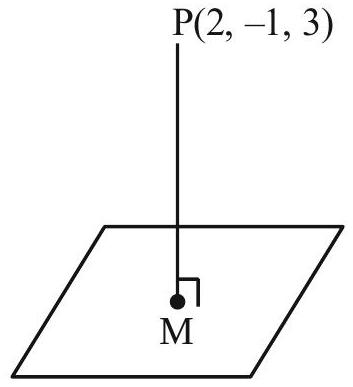
\includegraphics[max width=\textwidth, center]{2025_10_03_d195c8d2898bd93b94b0g-5}\\
eq. of line \(\mathrm{PM} \frac{x-2}{1}=\frac{y+1}{2}=\frac{z-3}{-1}=\lambda\)\\
any point on line \(=(\lambda+2,2 \lambda-1,-\lambda+3)\)\\
for point ' m ' \((\lambda+2)+2(2 \lambda-1)-(3-\lambda)=0\)

\[
\lambda=\frac{1}{2}
\]

Point m \(\left(\frac{1}{2}+2,2 \times \frac{1}{2}-1, \frac{-1}{2}+3\right)\)\\
\(=\left(\frac{5}{2}, 0, \frac{5}{2}\right)\)\\
For Image Q \((\alpha, \beta, \gamma)\)\\
\(\frac{\alpha+2}{2}=\frac{5}{2}, \frac{\beta-1}{2}=0\),\\
\(\frac{\gamma+3}{2}=\frac{5}{2}\)\\
Q : \((3,1,2)\)\\
\(\mathrm{d}=\left|\frac{3(3)+2(1)+2+29}{\sqrt{3^{2}+2^{2}+1^{2}}}\right|\)\\
\(\mathrm{d}=\frac{42}{\sqrt{14}}=3 \sqrt{14}\)\\
77. Let \(\quad \mathrm{f}(\mathrm{x})=\left|\begin{array}{ccc}1+\sin ^{2} \mathrm{x} & \cos ^{2} \mathrm{x} & \sin 2 \mathrm{x} \\ \sin ^{2} \mathrm{x} & 1+\cos ^{2} \mathrm{x} & \sin 2 \mathrm{x} \\ \sin ^{2} \mathrm{x} & \cos ^{2} \mathrm{x} & 1+\sin 2 \mathrm{x}\end{array}\right|\), \(\mathrm{x} \in\left[\frac{\pi}{6}, \frac{\pi}{3}\right]\). If \(\alpha\) a \(\beta\) respectively are the maximum and the minimum values of f , then\\
(1) \(\beta^{2}-2 \sqrt{\alpha}=\frac{19}{4}\)\\
(2) \(\beta^{2}+2 \sqrt{\alpha}=\frac{19}{4}\)\\
(3) \(\alpha^{2}-\beta^{2}=4 \sqrt{3}\)\\
(4) \(\alpha^{2}+\beta^{2}=\frac{9}{2}\)

Official Ans. by NTA (1)\\
Allen Ans. (1)\\
Sol.\\
\(\mathrm{C}_{1} \rightarrow \mathrm{C}_{1}+\mathrm{C}_{2}+\mathrm{C}_{3}\)\\
\(f(x)=\left|\begin{array}{ccc}2+\sin 2 x & \cos ^{2} x & \sin 2 x \\ 2+\sin 2 x & 1+\cos ^{2} x & \sin 2 x \\ 2+\sin 2 x & \cos ^{2} x & 1+\sin 2 x\end{array}\right|\)\\
\(f(x)=(2+\sin 2 x)\left|\begin{array}{ccc}1 & \cos ^{2} x & \sin 2 x \\ 1 & 1+\cos ^{2} x & \sin 2 x \\ 1 & \cos ^{2} x & 1+\sin 2 x\end{array}\right|\)\\
\(R_{2} \rightarrow R_{2}-R_{1}\)\\
\(R_{3} \rightarrow R_{3}-R_{1}\)\\
\(f(x)=2+\sin 2 x)\left|\begin{array}{ccc}1 & \cos ^{2} x & \sin 2 x \\ 0 & 1 & 0 \\ 0 & 0 & 1\end{array}\right|\)\\
\(=(2+\sin 2 \mathrm{x})(1)=2+\sin 2 \mathrm{x}\)\\
\(=\sin 2 x \in\left[\frac{\sqrt{3}}{2}, 1\right]\)\\
Hence \(2+\sin 2 x \in\left[2+\frac{\sqrt{3}}{2}, 3\right]\)\\
78. Let \(\mathrm{f}(\mathrm{x})=2 \mathrm{x}+\tan ^{-1} \mathrm{x}\) and \(\mathrm{g}(\mathrm{x})=\log _{\mathrm{e}}\left(\sqrt{1+\mathrm{x}^{2}}+\mathrm{x}\right)\), \(x \in[0,3]\). Then\\
(1) There exists \(\mathrm{x} \in[0,3]\) such that \(\mathrm{f}^{\prime}(\mathrm{x})<\mathrm{g}^{\prime}(\mathrm{x})\)\\
(2) max \(\mathrm{f}(\mathrm{x})>\max \mathrm{g}(\mathrm{x})\)\\
(3) There exist \(0<\mathrm{x}_{1}<\mathrm{x}_{2}<3\) such that \(\mathrm{f}(\mathrm{x})<\mathrm{g}(\mathrm{x})\), \(\forall \mathrm{x} \in\left(\mathrm{x}_{1}, \mathrm{x}_{2}\right)\)\\
(4) \(\min \mathrm{f}^{\prime}(\mathrm{x})=1+\max \mathrm{g}^{\prime}(\mathrm{x})\)

Official Ans. by NTA (2)\\
Allen Ans. (2)\\
Sol.\\
\(\mathrm{f}(\mathrm{x})=2 \mathrm{x}+\tan ^{-1} \mathrm{x}\) and \(\mathrm{g}(\mathrm{x})=\ln \left(\sqrt{1+x^{2}}+x\right)\)\\
and \(x \in[0,3]\)\\
\(\mathrm{g}^{\prime}(\mathrm{x})=\frac{1}{\sqrt{1+x^{2}}}\)\\
Now, \(0 \leq x \leq 3\)\\
\(0 \leq x^{2} \leq 9\)\\
\(1 \leq 1+x^{2} \leq 10\)\\
So, \(\quad 2+\frac{1}{10} \leq f^{\prime}(x) \leq 3\)\\
\(\frac{21}{10} \leq f^{\prime}(x) \leq 3\) and \(\frac{1}{\sqrt{10}} \leq g^{\prime}(x) \leq 1\)\\
option (4) is incorrect\\
From above, \(\mathrm{g}^{\prime}(\mathrm{x})<\mathrm{f}^{\prime}(\mathrm{x}) \forall \mathrm{x} \in[0,3]\)\\
Option (1) is incorrect.\\
\(\mathrm{f}^{\prime}(\mathrm{x}) \& \mathrm{~g}^{\prime}(\mathrm{x})\) both positive so \(\mathrm{f}(\mathrm{x}) \& \mathrm{~g}(\mathrm{x})\) both are increasing

So, \(\quad \max \left(\mathrm{f}(\mathrm{x})\right.\) at \(\mathrm{x}=3\) is \(6+\tan ^{-1} 3\)\\
\(\operatorname{Max}(\mathrm{g}(\mathrm{x})\) at \(\mathrm{x}=3\) is \(\ln (3+\sqrt{10})\)\\
And \(6+\tan ^{-1} 3>\ln (3+\sqrt{10})\)\\
Option (2) is correct\\
79. The mean and variance of 5 observations are 5 and 8 respectively. If 3 observations are \(1,3,5\), then the sum of cubes of the remaining two observations is\\
(1) 1072\\
(2) 1792\\
(3) 1216\\
(4) 1456

Official Ans. by NTA (1)\\
Allen Ans. (1)\\
Sol. \(\frac{1+3+5+\mathrm{a}+\mathrm{b}}{5}=5\)\\
\(a+b=16\) \(\_\_\_\_\)\\
\(\sigma^{2}=\frac{\sum \mathrm{x}_{1}^{2}}{5}-\left(\frac{\sum \mathrm{x}}{5}\right)^{2}\)\\
\(8=\frac{1^{2}+3^{2}+5^{2}+\mathrm{a}^{2}+\mathrm{b}^{2}}{5}-25\)\\
\(\mathrm{a}^{2}+\mathrm{b}^{2}=130\)\\
by (1), (2)\\
\(\mathrm{a}=7, \mathrm{~b}=9\)\\
or \(a=9, b=7\)\\
80. The area enclosed by the closed curve C given by the differential equation \(\frac{d y}{d x}+\frac{x+a}{y-2}=0, y(1)=0\) is \(4 \pi\).

Let P and Q be the points of intersection of the curve C and the y -axis. If normals at P and Q on the curve C intersect x -axis at points R and S respectively, then the length of the line segment RS is\\
(1) \(2 \sqrt{3}\)\\
(2) \(\frac{2 \sqrt{3}}{3}\)\\
(3) 2\\
(4) \(\frac{4 \sqrt{3}}{3}\)

Official Ans. by NTA (4)\\
Allen Ans. (4)\\
Sol. \(\frac{d y}{d x}+\frac{x+a}{y-2}=0\)\\
\(\frac{d y}{d x}=\frac{x+a}{2-y}\)\\
\((2-y) d y=(x+a) d x\)\\
\(2 y \frac{-y}{2}=\frac{x^{2}}{2}+\mathrm{ax}+\mathrm{c}\)\\
\(\mathrm{a}+\mathrm{c}=-\frac{1}{2}\) as \(\mathrm{y}(1)=0\)\\
\(X^{2}+y^{2}+2 a x-4 y-1-2 a=0\)\\
\(\pi \mathrm{r}^{2}=4 \pi\)\\
\(\mathrm{r}^{2}=4\)\\
\(4=\sqrt{a^{2}+4+1+2 a}\)\\
\((a+1)^{2}=0\)\\
\(\mathrm{P}, \mathrm{Q}=(0,2 \pm \sqrt{3})\)\\
Equation of normal at \(\mathrm{P}, \mathrm{Q}\) are \(\mathrm{y}-2=\sqrt{3}(\mathrm{x}-1)\)\\
\(y-2=-\sqrt{3}(x-1)\)\\
\(\mathrm{R}=\left(1-\frac{2}{\sqrt{3}}, 0\right)\)\\
\(S=\left(1+\frac{2}{\sqrt{3}}, 0\right)\)\\
\(R S=\frac{4}{\sqrt{3}}=4 \frac{\sqrt{3}}{3}\)

\section*{SECTION-B}
\begin{enumerate}
  \setcounter{enumi}{80}
  \item Let \(a_{1}=8, a_{2}, a_{3}, \ldots . a_{n}\) be an A.P. If the sum of its first four terms is 50 and the sum of its last four terms is 170 , then the product of its middle two terms is \(\_\_\_\_\) .\\
Official Ans. by NTA (754)\\
Allen Ans. (754)\\
Sol. \(\quad \mathrm{a}_{1}+\mathrm{a}_{2}+\mathrm{a}_{3}+\mathrm{a}_{4}=50\)\\
\(\Rightarrow 32+6 \mathrm{~d}=50\)\\
\(\Rightarrow \mathrm{d}=3\)\\
and, \(a_{n-3}+a_{n-2}+a_{n-1}+a_{n}=170\)\\
\(\Rightarrow 32+(4 \mathrm{n}-10) .3=170\)\\
\(\Rightarrow \mathrm{n}=14\)\\
\(\mathrm{a}_{7}=26, \mathrm{a}_{8}=29\)\\
\(\Rightarrow \mathrm{a}_{7} . \mathrm{a}_{8}=754\)
  \item \(\mathrm{A}(2,6,2), \mathrm{B}(-4,0, \lambda), \mathrm{C}(2,3,-1)\) and \(\mathrm{D}(4,5,0)\), \(|\lambda| \leq 5\) are the vertices of a quadrilateral ABCD . If its area is 18 square units, then \(5-6 \lambda\) is equal to\\
\(\_\_\_\_\) .\\
Official Ans. by NTA (11)\\
Allen Ans. (11)
\end{enumerate}

Sol. \(\mathrm{A}(2,6,2) \quad \mathrm{B}(-4,0, \lambda), \mathrm{C}(2,3,-1) \mathrm{D}(4,5,0)\)\\
Area \(=\frac{1}{2}|\overrightarrow{B D} \times \overrightarrow{A C}|=18\)\\
\(\overrightarrow{A C} \times \overrightarrow{B D}=\left|\begin{array}{ccc}\hat{i} & j & k \\ 0 & -3 & -3 \\ 8 & 5 & -\lambda\end{array}\right|\)\\
\(=(3 \lambda+15) \hat{i}-j(-24)+k(-24)\)\\
\(\overrightarrow{A C} \times \overrightarrow{B D}=(3 \lambda+15) \hat{i}+24 j-24 k\)\\
\(=\sqrt{(3 \lambda+15)^{2}+(24)^{2}+(24)^{2}}=36\)\\
\(=\lambda^{2}+10 \lambda+9=0\)\\
\(=\lambda=-1,-9\)\\
\(|\lambda| \leq 5 \Rightarrow \lambda=-1\)\\
\(5-6 \lambda=5-6(-1)=11\)\\
83. The number of 3-digit numbers, that are divisible by either 2 or 3 but not divisible by 7 is \(\_\_\_\_\) .\\
Official Ans. by NTA (514)\\
Allen Ans. (514)\\
Sol. Divisible by \(2 \rightarrow 450\)\\
Divisible by \(3 \rightarrow 300\)\\
Divisible by \(7 \rightarrow 128\)\\
Divisible by \(2 \& 7 \rightarrow 64\)\\
Divisible by \(3 \& 7 \rightarrow 43\)\\
Divisible by \(2 \& 3 \rightarrow 150\)\\
Divisible by \(2,3 \& 7 \rightarrow 21\)\\
\(\therefore\) Total numbers \(=450+300-150-64-43+21=514\)\\
84. The remainder when \(19^{200}+23^{200}\) is divided by 49 , is \(\_\_\_\_\)。\\
Official Ans. by NTA (29)\\
Allen Ans. (29)\\
Sol. \((21+2)^{200}+(21-2)^{200}\)\\
\(\Rightarrow 2\left[{ }^{100} \mathrm{C}_{0} 21^{200}+200 \mathrm{C}_{2} 21^{198} .2^{2}+\ldots . .+{ }^{200} \mathrm{C}_{198}\right.\)\\
\(\left.21^{2} .2^{198}+2^{200}\right]\)\\
\(\Rightarrow 2\left[49 \mathrm{I}_{1}+2^{200}\right]=49 \mathrm{I}_{1}+2^{201}\)\\
Now, \(2^{201}=(8)^{67}=(1+7)^{67}=49 \mathrm{I}_{2}+{ }^{67} \mathrm{C}_{0}{ }^{67} \mathrm{C}_{1} .7= 49 \mathrm{I}_{2}+470=49 \mathrm{I}_{2}+49 \times 9+29\)\\
\(\therefore\) Remainder is 29\\
85. If\\
\(\int_{0}^{1}\left(x^{21}+x^{14}+x^{7}\right)\left(2 x^{14}+3 x^{7}+6\right)^{1 / 7} d x=\frac{1}{l}(11)^{m / n}\)\\
where \(1, m, n \in \mathbb{N}, m\) and \(n\) are coprime then \(1+m+n\) is equal to \(\_\_\_\_\) .\\
Official Ans. by NTA (63)\\
Allen Ans. (63)\\
Sol. \(\int\left(x^{20}+x^{13}+x^{6}\right)\left(2 x^{21}+3 x^{14}+6 x^{7}\right)^{1 / 7} d x\)\\
\(2 \mathrm{x}^{21}+3 \mathrm{x}^{14}+6 \mathrm{x}^{7}=\mathrm{t}\)\\
\(42\left(x^{20}+x^{13}+x^{6}\right) d x=d t\)\\
\(\frac{1}{42} \int_{0}^{11} t^{\frac{1}{7}} d t=\left(\frac{t^{\frac{8}{7}}}{\frac{8}{7}} \times \frac{1}{42}\right)_{0}^{11}\)\\
\(=\frac{1}{48}\left(t^{\frac{8}{7}}\right)_{0}^{11}=\frac{1}{48}(11)^{8 / 7}\)

\[
\begin{aligned}
& l=48, \mathrm{~m}=8, \mathrm{n}=7 \\
& l+\mathrm{m}+\mathrm{n}=63
\end{aligned}
\]

\begin{enumerate}
  \setcounter{enumi}{85}
  \item If \(f(x)=x^{2}+g^{\prime}(1) x+g^{\prime \prime}(2)\) and
\end{enumerate}

\[
g(x)=f(1) x^{2}+x f^{\prime}(x)+f^{\prime \prime}(x),
\]

then the value of \(\mathrm{f}(4)-\mathrm{g}(4)\) is equal to \(\_\_\_\_\) .\\
Official Ans. by NTA (14)\\
Allen Ans. (14)\\
Sol. \(f(x)=x^{2}+g^{\prime}(1) x+g^{\prime \prime}(2)\)\\
\(\mathrm{f}^{\prime}(\mathrm{x})=2 \mathrm{x}+\mathrm{g}^{\prime}(1)\)\\
\(\mathrm{f}^{\prime \prime}(\mathrm{x})=2\)\\
\(\mathrm{g}(\mathrm{x})=\mathrm{f}(1) \mathrm{x}^{2}+\mathrm{x}\left[2 \mathrm{x}+\mathrm{g}^{\prime}(1)\right]+2\)\\
\(\mathrm{g}^{\prime}(\mathrm{x})=2 \mathrm{f}(1) \mathrm{x}+4 \mathrm{x}+\mathrm{g}^{\prime}(1)\)\\
\(\mathrm{g}^{\prime \prime}(\mathrm{x})=2 \mathrm{f}(1)+4\)\\
\(\mathrm{g}^{\prime \prime}(\mathrm{x})=0\)\\
\(2 \mathrm{f}(1)+4=0\)\\
\(f(1)=-2\)\\
\(-2=1+\mathrm{g}^{\prime}(1)=\mathrm{g}^{\prime}(1)=-3\)\\
So, \(\quad \mathrm{f}^{\prime}(\mathrm{x})=2 \mathrm{x}-3\)\\
\(f(x)=x^{2}-3 x+c\)\\
\(\mathrm{c}=0\)\\
\(f(x)=x^{2}-3 x\)\\
\(\mathrm{g}(\mathrm{x})=-3 \mathrm{x}+2\)\\
\(f(4)-g(4)=14\)\\
87. Let \(\vec{v}=\alpha \hat{i}+2 j-3 k, \vec{w}=2 \alpha \hat{i}+j-k\), and \(\vec{u}\) be a vector such that \(|\vec{u}|=\alpha>0\). If the minimum value of the scalar triple product \([\vec{u} \vec{v} \vec{w}]\) is \(-\alpha \sqrt{3401}\), and \(|\overrightarrow{\mathrm{u}} . \hat{\mathrm{i}}|^{2}=\frac{\mathrm{m}}{\mathrm{n}}\) where m and n are coprime natural numbers, then \(\mathrm{m}+\mathrm{n}\) is equal to \(\_\_\_\_\) .\\
Official Ans. by NTA (3501)\\
Allen Ans. (3501)\\
Sol. \([\vec{u} \vec{v} \vec{w}]=\vec{u} \cdot(\vec{v} \times \vec{w})\)\\
\(\min .(|u||\vec{v} \times \vec{w}| \cos \theta)=-\alpha \sqrt{3401}\)\\
\(\Rightarrow \quad \cos \theta=-1\)\\
\(|u|=\alpha\) (Given)\\
\(|\vec{v} \times \vec{w}|=\sqrt{3401}\)\\
\(\vec{v} \times \vec{w}=\left|\begin{array}{ccc}\hat{i} & j & k \\ \alpha & 2 & -3 \\ 2 \alpha & 1 & -1\end{array}\right|\)\\
\(\vec{v} \times \vec{w}=\hat{i}-5 \alpha j-3 \alpha k\)\\
\(|\vec{v} \times \vec{w}|=\sqrt{1+25 \alpha^{2}+9 \alpha^{2}}=\sqrt{3401}\)

\[
\begin{aligned}
& 34 \alpha^{2}=3400 \\
& \alpha^{2}=100 \\
& \alpha=10 \quad(\text { as } \alpha>0)
\end{aligned}
\]

So\\
\(\vec{u}=\lambda(\hat{i}-5 \alpha j-3 \alpha k)\)\\
\(\vec{u}=\sqrt{\lambda^{2}+25 \alpha^{2} \lambda^{2}+9 \alpha^{2} \lambda}\)\\
\(\alpha^{2}=\lambda^{2}\left(1+25 \alpha^{2}+9 \alpha^{2}\right)\)\\
\(100=\lambda^{2}(1+34 \times 100)\)\\
\(\lambda^{2}=\frac{100}{3401}=\frac{m}{n}\)\\
88. The number of words, with or without meaning, that can be formed using all the letters of the word ASSASSINATION so that the vowels occur together, is \(\_\_\_\_\) .\\
Official Ans. by NTA (50400)\\
Allen Ans. (50400)

Sol. Vowels : A,A,A,I,I,O\\
Consonants : S,S,S,S,N,N,T\\
\(\square\) Total number of ways in which vowels come together\\
\(=\frac{\underline{8}}{\underline{4} \underline{2}} \times \frac{\underline{6}}{\underline{3} \underline{2}}=50400\)\\
89. Let A be the area bounded by the curve \(\mathrm{y}=\mathrm{x}|\mathrm{x}-3|\), the x -axis and the ordinates \(\mathrm{x}=-1\) and \(x=2\). Then 12 A is equal to \(\_\_\_\_\) .\\
Official Ans. by NTA (62)\\
Allen Ans. (62)\\
Sol. \(\quad \mathrm{A}=\int_{-1}^{0}\left(\mathrm{x}^{2}-3 \mathrm{x}\right) \mathrm{dx}+\int_{0}^{2}\left(3 \mathrm{x}-\mathrm{x}^{2}\right) \mathrm{dx}\)\\
\(\Rightarrow \quad \mathrm{A}=\frac{\mathrm{x}^{3}}{3}-\left.\frac{3 \mathrm{x}^{2}}{2}\right|_{-1} ^{0}+\frac{3 \mathrm{x}^{2}}{2}-\left.\frac{\mathrm{x}^{3}}{3}\right|_{0} ^{2}\)\\
\(\Rightarrow \mathrm{A}=\frac{11}{6}+\frac{10}{3}=\frac{31}{6}\)\\
\(\therefore \quad 12 \mathrm{~A}=62\)\\
90. Let \(f: \mathbb{R} \rightarrow \mathbb{R}\) be a differentiable function such that \(f^{\prime}(x)+f(x)=\int_{0}^{2} f(t) d t\). If \(f(0)=e^{-2}\), then \(2 f(0)-f(2)\) is equal to \(\_\_\_\_\) .\\
Official Ans. by NTA (1)\\
Allen Ans. (1)\\
Sol. \(\frac{d y}{d x}+y=k\)

\[
\begin{array}{ll} 
& y \cdot e^{x}=k \cdot e^{x}+c \\
& f(0)=e^{-2} \\
\Rightarrow \quad & c=e^{-2}-k \\
\therefore \quad & y=k+\left(e^{-2}-k\right) e^{-x} \\
& \text { now } k=\int_{0}^{2}\left(k+\left(e^{-2}-k\right) e^{-x}\right) d x \\
\Rightarrow \quad & k=e^{-2}-1 \\
\therefore \quad & y=\left(e^{-2}-1\right)+e^{-x} \\
& f(2)=2 e^{-2}-1, f(0)=e^{-2} \\
& 2 f(0)-f(2)=1
\end{array}
\]


\end{document}